%\documentclass[draft]{beamer}%\documentclass[]{beamer}
\documentclass[]{beamer}%\documentclass[draft]{beamer}
\mode<presentation>
{
%  \usetheme{Boadilla}
  \usetheme{Frankfurt}
  \usecolortheme{crane}
}
\usepackage{graphicx}
\usepackage{amsmath}
\usepackage{url}
\setbeamerfont{fig_font}{size=\small}
\setbeamercovered{invisible}
\usefonttheme[onlysmall]{structurebold}

\AtBeginSection[]
{
  \begin{frame}<beamer>{Outline}
	\tableofcontents[currentsection]
  \end{frame}
}
 \AtBeginSubsection[]
 {
   \begin{frame}<beamer>{Outline}
     \tableofcontents[currentsection,currentsubsection]
   \end{frame}
 }

\title{Seat Allocation project : A CS251 Report by Group 02}
\author{Rohan Rathod \space 130050002 \\
	rohanrathod8758@gmail.com\\
	Chandra Mohan Soni \space 130050020 \\
	chandramohan.soni@gmail.com\\
	Ayush Dhakar \space 130050033\\
	ayushdhaker@gmail.com
	}
\date{October 31, 2014}
% End Beamer stuff
\begin{document}
\begin{frame}
\titlepage
Seat Allocation Project 
\end{frame}

\section{Introduction}
\begin{frame}
\frametitle{Introduction}
This report explains the details of our seat allocation project and features of it.
This project is about registering students in different colleges according to their ranks and create a web application framework to make them fill their preference list of choices of courses.
\end{frame}
\section{Body}
\subsection{Part1: Java }
\begin{frame}
\frametitle{Part1: Java}
 Implementation of algorithm using java  \\  \pause  User enters the information like Unique id, choices, category preferences, and additional information.\\  \pause We have created functions to manipluate all the data. \\   \pause There are 4 classes \\ 1. Candidate \\ 2. VirtualProgramme \\ 3. MeritList \\ 4. GaleShapleyAdmission \\ \pause


\end{frame}
\begin{frame}
\frametitle{Part1: Java }
 There are 2 algorithms used here.  \\ 1. Modified Gale- Shapely Stable Matching Algorithm \\ 2. Merit List order Allocation\pause


\end{frame}

\subsection{Part2: Python }
\begin{frame}
\frametitle{Part2: Python }
Used pdftotext to convert the pdf into a text file \\ \pause

There 2 file p1.py and update.py to take the input from HTML and .txt file and store it into a CSV  \\ \pause

The csv file has names of colleges, branches and branch codes

% \includegraphics[width = 0.75in,height = 1in]{rot.jpg}
\end{frame}

\subsection{Part 3 : Django }
\begin{frame}
\frametitle{Part 3 : Django}
Django is a high-level Python Web framework that encourages rapid development and clean, pragmatic design \\ \pause
Django is used for web interactive interface\\ \pause
In the context of project,  \\ \pause
It has 2 interfaces \\ \pause
1. Login Interface \\ \pause
2. Candidate preference choice selection interface


%\includegraphics[width = 1in,height = 0.75in]{pul.jpg}

\end{frame}
\begin{frame}
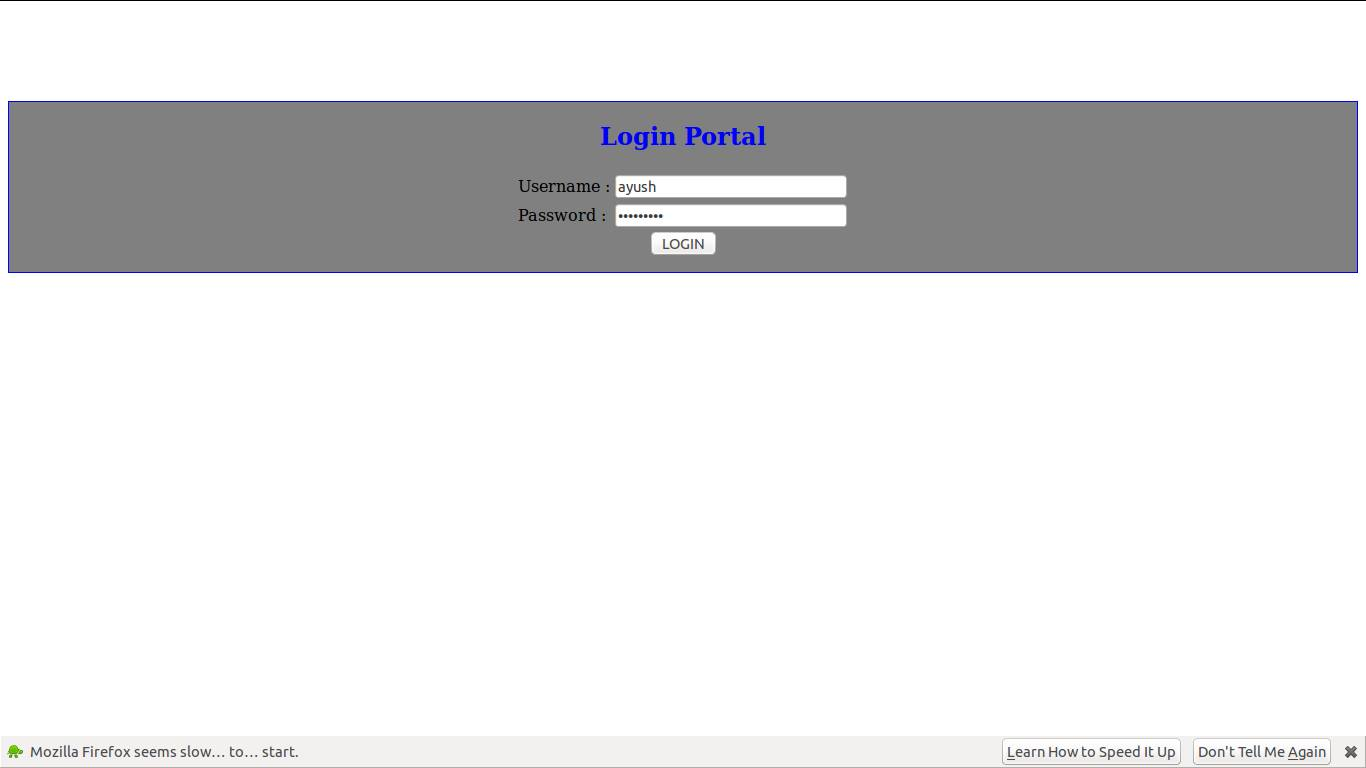
\includegraphics[width = 2in,height = 1.4in]{login.jpg}
This is the first web interface login page. The user enters the username and password assigned to him to make him fill his/her preferences choice.It handles all types of exceptions too.
\end{frame}


\begin{frame}
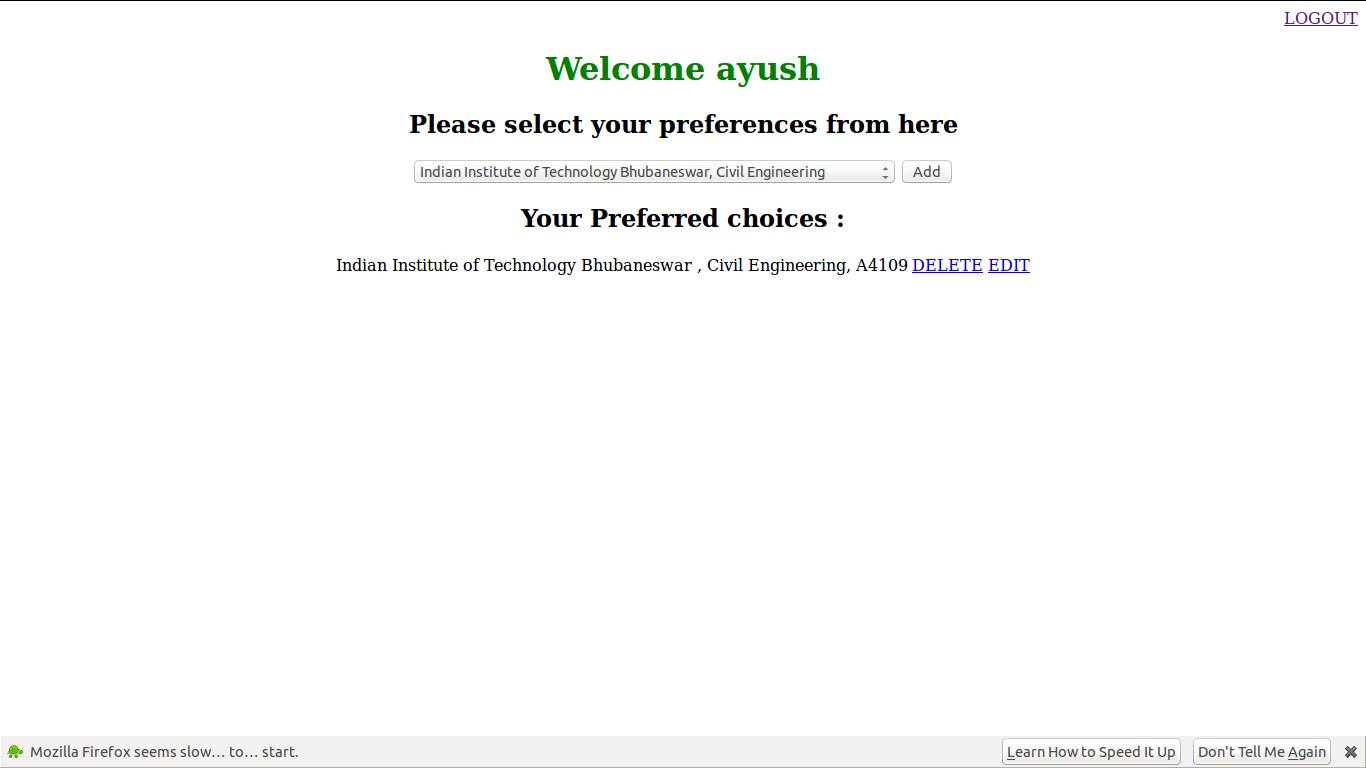
\includegraphics[width = 2in,height = 1.4in]{result.jpg}
This is the web interface for filling preferences by candidates.
The candidate is allowed to choose from dropdown list of courses. He can choose as many courses as he wants.
This also handles exceptions like filling two courses, having two courses become same on editing,etc. 
This also allows to modify preference list by various operations like edit and delete.
\end{frame}
\section{Conclusion}
\begin{frame}
\frametitle{Conclusion}
In conclusion we would like to point out some important points \\ \pause
1. Gale Shapley algorithm provides better solution to the seat allocation problem than the merit list alllocation concept. \\ \pause
2. However merit list allocation concept works faster than Gale Shapley algorithm implementation \\ \pause
3. We can make interactive web interface using Django very easily \\ \pause 
\end{frame}

\begin{frame}
\frametitle{References}
\footnotesize{
\begin{thebibliography}{99}
\bibitem{p1} Str!kers
\newblock \emph{Stack Overflow}
\newblock \emph{Syntax from Google}
\bibliographystyle{plain}
\bibliography{ref}
\end{thebibliography}
}
\end{frame}


\end{document}
